
\documentclass{article} % For LaTeX2e
\usepackage{iclr2024_conference,times}

% Optional math commands from https://github.com/goodfeli/dlbook_notation.
%%%%% NEW MATH DEFINITIONS %%%%%

\usepackage{amsmath,amsfonts,bm}

% Mark sections of captions for referring to divisions of figures
\newcommand{\figleft}{{\em (Left)}}
\newcommand{\figcenter}{{\em (Center)}}
\newcommand{\figright}{{\em (Right)}}
\newcommand{\figtop}{{\em (Top)}}
\newcommand{\figbottom}{{\em (Bottom)}}
\newcommand{\captiona}{{\em (a)}}
\newcommand{\captionb}{{\em (b)}}
\newcommand{\captionc}{{\em (c)}}
\newcommand{\captiond}{{\em (d)}}

% Highlight a newly defined term
\newcommand{\newterm}[1]{{\bf #1}}


% Figure reference, lower-case.
\def\figref#1{figure~\ref{#1}}
% Figure reference, capital. For start of sentence
\def\Figref#1{Figure~\ref{#1}}
\def\twofigref#1#2{figures \ref{#1} and \ref{#2}}
\def\quadfigref#1#2#3#4{figures \ref{#1}, \ref{#2}, \ref{#3} and \ref{#4}}
% Section reference, lower-case.
\def\secref#1{section~\ref{#1}}
% Section reference, capital.
\def\Secref#1{Section~\ref{#1}}
% Reference to two sections.
\def\twosecrefs#1#2{sections \ref{#1} and \ref{#2}}
% Reference to three sections.
\def\secrefs#1#2#3{sections \ref{#1}, \ref{#2} and \ref{#3}}
% Reference to an equation, lower-case.
\def\eqref#1{equation~\ref{#1}}
% Reference to an equation, upper case
\def\Eqref#1{Equation~\ref{#1}}
% A raw reference to an equation---avoid using if possible
\def\plaineqref#1{\ref{#1}}
% Reference to a chapter, lower-case.
\def\chapref#1{chapter~\ref{#1}}
% Reference to an equation, upper case.
\def\Chapref#1{Chapter~\ref{#1}}
% Reference to a range of chapters
\def\rangechapref#1#2{chapters\ref{#1}--\ref{#2}}
% Reference to an algorithm, lower-case.
\def\algref#1{algorithm~\ref{#1}}
% Reference to an algorithm, upper case.
\def\Algref#1{Algorithm~\ref{#1}}
\def\twoalgref#1#2{algorithms \ref{#1} and \ref{#2}}
\def\Twoalgref#1#2{Algorithms \ref{#1} and \ref{#2}}
% Reference to a part, lower case
\def\partref#1{part~\ref{#1}}
% Reference to a part, upper case
\def\Partref#1{Part~\ref{#1}}
\def\twopartref#1#2{parts \ref{#1} and \ref{#2}}

\def\ceil#1{\lceil #1 \rceil}
\def\floor#1{\lfloor #1 \rfloor}
\def\1{\bm{1}}
\newcommand{\train}{\mathcal{D}}
\newcommand{\valid}{\mathcal{D_{\mathrm{valid}}}}
\newcommand{\test}{\mathcal{D_{\mathrm{test}}}}

\def\eps{{\epsilon}}


% Random variables
\def\reta{{\textnormal{$\eta$}}}
\def\ra{{\textnormal{a}}}
\def\rb{{\textnormal{b}}}
\def\rc{{\textnormal{c}}}
\def\rd{{\textnormal{d}}}
\def\re{{\textnormal{e}}}
\def\rf{{\textnormal{f}}}
\def\rg{{\textnormal{g}}}
\def\rh{{\textnormal{h}}}
\def\ri{{\textnormal{i}}}
\def\rj{{\textnormal{j}}}
\def\rk{{\textnormal{k}}}
\def\rl{{\textnormal{l}}}
% rm is already a command, just don't name any random variables m
\def\rn{{\textnormal{n}}}
\def\ro{{\textnormal{o}}}
\def\rp{{\textnormal{p}}}
\def\rq{{\textnormal{q}}}
\def\rr{{\textnormal{r}}}
\def\rs{{\textnormal{s}}}
\def\rt{{\textnormal{t}}}
\def\ru{{\textnormal{u}}}
\def\rv{{\textnormal{v}}}
\def\rw{{\textnormal{w}}}
\def\rx{{\textnormal{x}}}
\def\ry{{\textnormal{y}}}
\def\rz{{\textnormal{z}}}

% Random vectors
\def\rvepsilon{{\mathbf{\epsilon}}}
\def\rvtheta{{\mathbf{\theta}}}
\def\rva{{\mathbf{a}}}
\def\rvb{{\mathbf{b}}}
\def\rvc{{\mathbf{c}}}
\def\rvd{{\mathbf{d}}}
\def\rve{{\mathbf{e}}}
\def\rvf{{\mathbf{f}}}
\def\rvg{{\mathbf{g}}}
\def\rvh{{\mathbf{h}}}
\def\rvu{{\mathbf{i}}}
\def\rvj{{\mathbf{j}}}
\def\rvk{{\mathbf{k}}}
\def\rvl{{\mathbf{l}}}
\def\rvm{{\mathbf{m}}}
\def\rvn{{\mathbf{n}}}
\def\rvo{{\mathbf{o}}}
\def\rvp{{\mathbf{p}}}
\def\rvq{{\mathbf{q}}}
\def\rvr{{\mathbf{r}}}
\def\rvs{{\mathbf{s}}}
\def\rvt{{\mathbf{t}}}
\def\rvu{{\mathbf{u}}}
\def\rvv{{\mathbf{v}}}
\def\rvw{{\mathbf{w}}}
\def\rvx{{\mathbf{x}}}
\def\rvy{{\mathbf{y}}}
\def\rvz{{\mathbf{z}}}

% Elements of random vectors
\def\erva{{\textnormal{a}}}
\def\ervb{{\textnormal{b}}}
\def\ervc{{\textnormal{c}}}
\def\ervd{{\textnormal{d}}}
\def\erve{{\textnormal{e}}}
\def\ervf{{\textnormal{f}}}
\def\ervg{{\textnormal{g}}}
\def\ervh{{\textnormal{h}}}
\def\ervi{{\textnormal{i}}}
\def\ervj{{\textnormal{j}}}
\def\ervk{{\textnormal{k}}}
\def\ervl{{\textnormal{l}}}
\def\ervm{{\textnormal{m}}}
\def\ervn{{\textnormal{n}}}
\def\ervo{{\textnormal{o}}}
\def\ervp{{\textnormal{p}}}
\def\ervq{{\textnormal{q}}}
\def\ervr{{\textnormal{r}}}
\def\ervs{{\textnormal{s}}}
\def\ervt{{\textnormal{t}}}
\def\ervu{{\textnormal{u}}}
\def\ervv{{\textnormal{v}}}
\def\ervw{{\textnormal{w}}}
\def\ervx{{\textnormal{x}}}
\def\ervy{{\textnormal{y}}}
\def\ervz{{\textnormal{z}}}

% Random matrices
\def\rmA{{\mathbf{A}}}
\def\rmB{{\mathbf{B}}}
\def\rmC{{\mathbf{C}}}
\def\rmD{{\mathbf{D}}}
\def\rmE{{\mathbf{E}}}
\def\rmF{{\mathbf{F}}}
\def\rmG{{\mathbf{G}}}
\def\rmH{{\mathbf{H}}}
\def\rmI{{\mathbf{I}}}
\def\rmJ{{\mathbf{J}}}
\def\rmK{{\mathbf{K}}}
\def\rmL{{\mathbf{L}}}
\def\rmM{{\mathbf{M}}}
\def\rmN{{\mathbf{N}}}
\def\rmO{{\mathbf{O}}}
\def\rmP{{\mathbf{P}}}
\def\rmQ{{\mathbf{Q}}}
\def\rmR{{\mathbf{R}}}
\def\rmS{{\mathbf{S}}}
\def\rmT{{\mathbf{T}}}
\def\rmU{{\mathbf{U}}}
\def\rmV{{\mathbf{V}}}
\def\rmW{{\mathbf{W}}}
\def\rmX{{\mathbf{X}}}
\def\rmY{{\mathbf{Y}}}
\def\rmZ{{\mathbf{Z}}}

% Elements of random matrices
\def\ermA{{\textnormal{A}}}
\def\ermB{{\textnormal{B}}}
\def\ermC{{\textnormal{C}}}
\def\ermD{{\textnormal{D}}}
\def\ermE{{\textnormal{E}}}
\def\ermF{{\textnormal{F}}}
\def\ermG{{\textnormal{G}}}
\def\ermH{{\textnormal{H}}}
\def\ermI{{\textnormal{I}}}
\def\ermJ{{\textnormal{J}}}
\def\ermK{{\textnormal{K}}}
\def\ermL{{\textnormal{L}}}
\def\ermM{{\textnormal{M}}}
\def\ermN{{\textnormal{N}}}
\def\ermO{{\textnormal{O}}}
\def\ermP{{\textnormal{P}}}
\def\ermQ{{\textnormal{Q}}}
\def\ermR{{\textnormal{R}}}
\def\ermS{{\textnormal{S}}}
\def\ermT{{\textnormal{T}}}
\def\ermU{{\textnormal{U}}}
\def\ermV{{\textnormal{V}}}
\def\ermW{{\textnormal{W}}}
\def\ermX{{\textnormal{X}}}
\def\ermY{{\textnormal{Y}}}
\def\ermZ{{\textnormal{Z}}}

% Vectors
\def\vzero{{\bm{0}}}
\def\vone{{\bm{1}}}
\def\vmu{{\bm{\mu}}}
\def\vtheta{{\bm{\theta}}}
\def\va{{\bm{a}}}
\def\vb{{\bm{b}}}
\def\vc{{\bm{c}}}
\def\vd{{\bm{d}}}
\def\ve{{\bm{e}}}
\def\vf{{\bm{f}}}
\def\vg{{\bm{g}}}
\def\vh{{\bm{h}}}
\def\vi{{\bm{i}}}
\def\vj{{\bm{j}}}
\def\vk{{\bm{k}}}
\def\vl{{\bm{l}}}
\def\vm{{\bm{m}}}
\def\vn{{\bm{n}}}
\def\vo{{\bm{o}}}
\def\vp{{\bm{p}}}
\def\vq{{\bm{q}}}
\def\vr{{\bm{r}}}
\def\vs{{\bm{s}}}
\def\vt{{\bm{t}}}
\def\vu{{\bm{u}}}
\def\vv{{\bm{v}}}
\def\vw{{\bm{w}}}
\def\vx{{\bm{x}}}
\def\vy{{\bm{y}}}
\def\vz{{\bm{z}}}

% Elements of vectors
\def\evalpha{{\alpha}}
\def\evbeta{{\beta}}
\def\evepsilon{{\epsilon}}
\def\evlambda{{\lambda}}
\def\evomega{{\omega}}
\def\evmu{{\mu}}
\def\evpsi{{\psi}}
\def\evsigma{{\sigma}}
\def\evtheta{{\theta}}
\def\eva{{a}}
\def\evb{{b}}
\def\evc{{c}}
\def\evd{{d}}
\def\eve{{e}}
\def\evf{{f}}
\def\evg{{g}}
\def\evh{{h}}
\def\evi{{i}}
\def\evj{{j}}
\def\evk{{k}}
\def\evl{{l}}
\def\evm{{m}}
\def\evn{{n}}
\def\evo{{o}}
\def\evp{{p}}
\def\evq{{q}}
\def\evr{{r}}
\def\evs{{s}}
\def\evt{{t}}
\def\evu{{u}}
\def\evv{{v}}
\def\evw{{w}}
\def\evx{{x}}
\def\evy{{y}}
\def\evz{{z}}

% Matrix
\def\mA{{\bm{A}}}
\def\mB{{\bm{B}}}
\def\mC{{\bm{C}}}
\def\mD{{\bm{D}}}
\def\mE{{\bm{E}}}
\def\mF{{\bm{F}}}
\def\mG{{\bm{G}}}
\def\mH{{\bm{H}}}
\def\mI{{\bm{I}}}
\def\mJ{{\bm{J}}}
\def\mK{{\bm{K}}}
\def\mL{{\bm{L}}}
\def\mM{{\bm{M}}}
\def\mN{{\bm{N}}}
\def\mO{{\bm{O}}}
\def\mP{{\bm{P}}}
\def\mQ{{\bm{Q}}}
\def\mR{{\bm{R}}}
\def\mS{{\bm{S}}}
\def\mT{{\bm{T}}}
\def\mU{{\bm{U}}}
\def\mV{{\bm{V}}}
\def\mW{{\bm{W}}}
\def\mX{{\bm{X}}}
\def\mY{{\bm{Y}}}
\def\mZ{{\bm{Z}}}
\def\mBeta{{\bm{\beta}}}
\def\mPhi{{\bm{\Phi}}}
\def\mLambda{{\bm{\Lambda}}}
\def\mSigma{{\bm{\Sigma}}}

% Tensor
\DeclareMathAlphabet{\mathsfit}{\encodingdefault}{\sfdefault}{m}{sl}
\SetMathAlphabet{\mathsfit}{bold}{\encodingdefault}{\sfdefault}{bx}{n}
\newcommand{\tens}[1]{\bm{\mathsfit{#1}}}
\def\tA{{\tens{A}}}
\def\tB{{\tens{B}}}
\def\tC{{\tens{C}}}
\def\tD{{\tens{D}}}
\def\tE{{\tens{E}}}
\def\tF{{\tens{F}}}
\def\tG{{\tens{G}}}
\def\tH{{\tens{H}}}
\def\tI{{\tens{I}}}
\def\tJ{{\tens{J}}}
\def\tK{{\tens{K}}}
\def\tL{{\tens{L}}}
\def\tM{{\tens{M}}}
\def\tN{{\tens{N}}}
\def\tO{{\tens{O}}}
\def\tP{{\tens{P}}}
\def\tQ{{\tens{Q}}}
\def\tR{{\tens{R}}}
\def\tS{{\tens{S}}}
\def\tT{{\tens{T}}}
\def\tU{{\tens{U}}}
\def\tV{{\tens{V}}}
\def\tW{{\tens{W}}}
\def\tX{{\tens{X}}}
\def\tY{{\tens{Y}}}
\def\tZ{{\tens{Z}}}


% Graph
\def\gA{{\mathcal{A}}}
\def\gB{{\mathcal{B}}}
\def\gC{{\mathcal{C}}}
\def\gD{{\mathcal{D}}}
\def\gE{{\mathcal{E}}}
\def\gF{{\mathcal{F}}}
\def\gG{{\mathcal{G}}}
\def\gH{{\mathcal{H}}}
\def\gI{{\mathcal{I}}}
\def\gJ{{\mathcal{J}}}
\def\gK{{\mathcal{K}}}
\def\gL{{\mathcal{L}}}
\def\gM{{\mathcal{M}}}
\def\gN{{\mathcal{N}}}
\def\gO{{\mathcal{O}}}
\def\gP{{\mathcal{P}}}
\def\gQ{{\mathcal{Q}}}
\def\gR{{\mathcal{R}}}
\def\gS{{\mathcal{S}}}
\def\gT{{\mathcal{T}}}
\def\gU{{\mathcal{U}}}
\def\gV{{\mathcal{V}}}
\def\gW{{\mathcal{W}}}
\def\gX{{\mathcal{X}}}
\def\gY{{\mathcal{Y}}}
\def\gZ{{\mathcal{Z}}}

% Sets
\def\sA{{\mathbb{A}}}
\def\sB{{\mathbb{B}}}
\def\sC{{\mathbb{C}}}
\def\sD{{\mathbb{D}}}
% Don't use a set called E, because this would be the same as our symbol
% for expectation.
\def\sF{{\mathbb{F}}}
\def\sG{{\mathbb{G}}}
\def\sH{{\mathbb{H}}}
\def\sI{{\mathbb{I}}}
\def\sJ{{\mathbb{J}}}
\def\sK{{\mathbb{K}}}
\def\sL{{\mathbb{L}}}
\def\sM{{\mathbb{M}}}
\def\sN{{\mathbb{N}}}
\def\sO{{\mathbb{O}}}
\def\sP{{\mathbb{P}}}
\def\sQ{{\mathbb{Q}}}
\def\sR{{\mathbb{R}}}
\def\sS{{\mathbb{S}}}
\def\sT{{\mathbb{T}}}
\def\sU{{\mathbb{U}}}
\def\sV{{\mathbb{V}}}
\def\sW{{\mathbb{W}}}
\def\sX{{\mathbb{X}}}
\def\sY{{\mathbb{Y}}}
\def\sZ{{\mathbb{Z}}}

% Entries of a matrix
\def\emLambda{{\Lambda}}
\def\emA{{A}}
\def\emB{{B}}
\def\emC{{C}}
\def\emD{{D}}
\def\emE{{E}}
\def\emF{{F}}
\def\emG{{G}}
\def\emH{{H}}
\def\emI{{I}}
\def\emJ{{J}}
\def\emK{{K}}
\def\emL{{L}}
\def\emM{{M}}
\def\emN{{N}}
\def\emO{{O}}
\def\emP{{P}}
\def\emQ{{Q}}
\def\emR{{R}}
\def\emS{{S}}
\def\emT{{T}}
\def\emU{{U}}
\def\emV{{V}}
\def\emW{{W}}
\def\emX{{X}}
\def\emY{{Y}}
\def\emZ{{Z}}
\def\emSigma{{\Sigma}}

% entries of a tensor
% Same font as tensor, without \bm wrapper
\newcommand{\etens}[1]{\mathsfit{#1}}
\def\etLambda{{\etens{\Lambda}}}
\def\etA{{\etens{A}}}
\def\etB{{\etens{B}}}
\def\etC{{\etens{C}}}
\def\etD{{\etens{D}}}
\def\etE{{\etens{E}}}
\def\etF{{\etens{F}}}
\def\etG{{\etens{G}}}
\def\etH{{\etens{H}}}
\def\etI{{\etens{I}}}
\def\etJ{{\etens{J}}}
\def\etK{{\etens{K}}}
\def\etL{{\etens{L}}}
\def\etM{{\etens{M}}}
\def\etN{{\etens{N}}}
\def\etO{{\etens{O}}}
\def\etP{{\etens{P}}}
\def\etQ{{\etens{Q}}}
\def\etR{{\etens{R}}}
\def\etS{{\etens{S}}}
\def\etT{{\etens{T}}}
\def\etU{{\etens{U}}}
\def\etV{{\etens{V}}}
\def\etW{{\etens{W}}}
\def\etX{{\etens{X}}}
\def\etY{{\etens{Y}}}
\def\etZ{{\etens{Z}}}

% The true underlying data generating distribution
\newcommand{\pdata}{p_{\rm{data}}}
% The empirical distribution defined by the training set
\newcommand{\ptrain}{\hat{p}_{\rm{data}}}
\newcommand{\Ptrain}{\hat{P}_{\rm{data}}}
% The model distribution
\newcommand{\pmodel}{p_{\rm{model}}}
\newcommand{\Pmodel}{P_{\rm{model}}}
\newcommand{\ptildemodel}{\tilde{p}_{\rm{model}}}
% Stochastic autoencoder distributions
\newcommand{\pencode}{p_{\rm{encoder}}}
\newcommand{\pdecode}{p_{\rm{decoder}}}
\newcommand{\precons}{p_{\rm{reconstruct}}}

\newcommand{\laplace}{\mathrm{Laplace}} % Laplace distribution

\newcommand{\E}{\mathbb{E}}
\newcommand{\Ls}{\mathcal{L}}
\newcommand{\R}{\mathbb{R}}
\newcommand{\emp}{\tilde{p}}
\newcommand{\lr}{\alpha}
\newcommand{\reg}{\lambda}
\newcommand{\rect}{\mathrm{rectifier}}
\newcommand{\softmax}{\mathrm{softmax}}
\newcommand{\sigmoid}{\sigma}
\newcommand{\softplus}{\zeta}
\newcommand{\KL}{D_{\mathrm{KL}}}
\newcommand{\Var}{\mathrm{Var}}
\newcommand{\standarderror}{\mathrm{SE}}
\newcommand{\Cov}{\mathrm{Cov}}
% Wolfram Mathworld says $L^2$ is for function spaces and $\ell^2$ is for vectors
% But then they seem to use $L^2$ for vectors throughout the site, and so does
% wikipedia.
\newcommand{\normlzero}{L^0}
\newcommand{\normlone}{L^1}
\newcommand{\normltwo}{L^2}
\newcommand{\normlp}{L^p}
\newcommand{\normmax}{L^\infty}

\newcommand{\parents}{Pa} % See usage in notation.tex. Chosen to match Daphne's book.

\DeclareMathOperator*{\argmax}{arg\,max}
\DeclareMathOperator*{\argmin}{arg\,min}

\DeclareMathOperator{\sign}{sign}
\DeclareMathOperator{\Tr}{Tr}
\let\ab\allowbreak


\usepackage{natbib}
\usepackage{hyperref}
\usepackage{graphicx}
\usepackage{url}
\usepackage{tikz}

\title{Neural Processes for Climate Emulation}

% Authors must not appear in the submitted version. They should be hidden
% as long as the \iclrfinalcopy macro remains commented out below.
% Non-anonymous submissions will be rejected without review.

\author{Jack Kai Lim 
\thanks{ Use footnote for providing further information
about author (webpage, alternative address)---\emph{not} for acknowledging
funding agencies.  Funding acknowledgements go at the end of the paper.} \\
Halıcıoğlu Data Science Institute\\
University of California, San Diego\\
\texttt{jklim@ucsd.edu} \\
}

% The \author macro works with any number of authors. There are two commands
% used to separate the names and addresses of multiple authors: \And and \AND.
%
% Using \And between authors leaves it to \LaTeX{} to determine where to break
% the lines. Using \AND forces a linebreak at that point. So, if \LaTeX{}
% puts 3 of 4 authors names on the first line, and the last on the second
% line, try using \AND instead of \And before the third author name.

\newcommand{\fix}{\marginpar{FIX}}
\newcommand{\new}{\marginpar{NEW}}

\iclrfinalcopy % Uncomment for camera-ready version, but NOT for submission.
\begin{document}


\maketitle

\begin{abstract}
   {Climate modeling has long been limited by the amount of resources needed to use legacy built Earth system models. As such, exploration into the many different and possible emission pathways have been relegated to one-dimensional impulse response or simple pattern scaling models, neither of which are capable of accounting for finer details when emulating the Shared Socioeconomic Pathways. This paper introduces a new benchmark using a (think of a word) model called a Neural Process in the hopes to improve upon the benchmarks that have been established in \cite{watson2022climatebench}. In the hopes that these Deep Learning models are capable of emulating the response of the full complexity of the Earth System Models to forcers using a fraction of the time and resources while also being more complex then simple pattern scaling models. These models would predict annualglobal mean global distributions of temperature, diurnal temperature range and precipitation given the emmisions and concentrations of Carbon Dioxide (C)$_2$, Methane (CH$_4$), Sulfur Dioxide (SO$_2$) and Black Carbon (BC).
    }
\end{abstract}

\section{Introduction}
Climate Scientist have already generated different emission pathways that are used to predict the future climate. These pathways are called the Shared Socioeconomic Pathways (SSPs). However, these models are computationally expensive and require a lot of resources to run, which limits the amount of exploration that can be done. Which is specifically important for policymakers as they need to assess different social and economic impacts under different emission scenarios to reduce the effect of climate change and achieve the goal. \cite{watson2022climatebench} introduced a benchmark using different machine learning models that emulate different emissions scenarios are able to generate predictions of global temperature, diurnal temperature, and precipitation(including extreme precipitation). This paper looks to build upon it by intorducing a new benchmark using a Neural Process model.

For the task at hand, we looked into a few implementations. A base Neural Process (NP) model \cite{gordon2020convolutional} which takes a sparse representation of the data and learns the distribution of the data. A Covolutional Neural Process (CNP) which introduces the use of Covolutional layer in the Neural Process, allowing the model to learn the spatial dependencies of the data and also a CNP which introduces the use of a Spherical Covolutional layer in the Neural Process, allowing the model to learn the spatial dependencies of the data in a spherical manner which fits the idea of the Earth being a sphere.

\begin{figure}
    \centering
     {{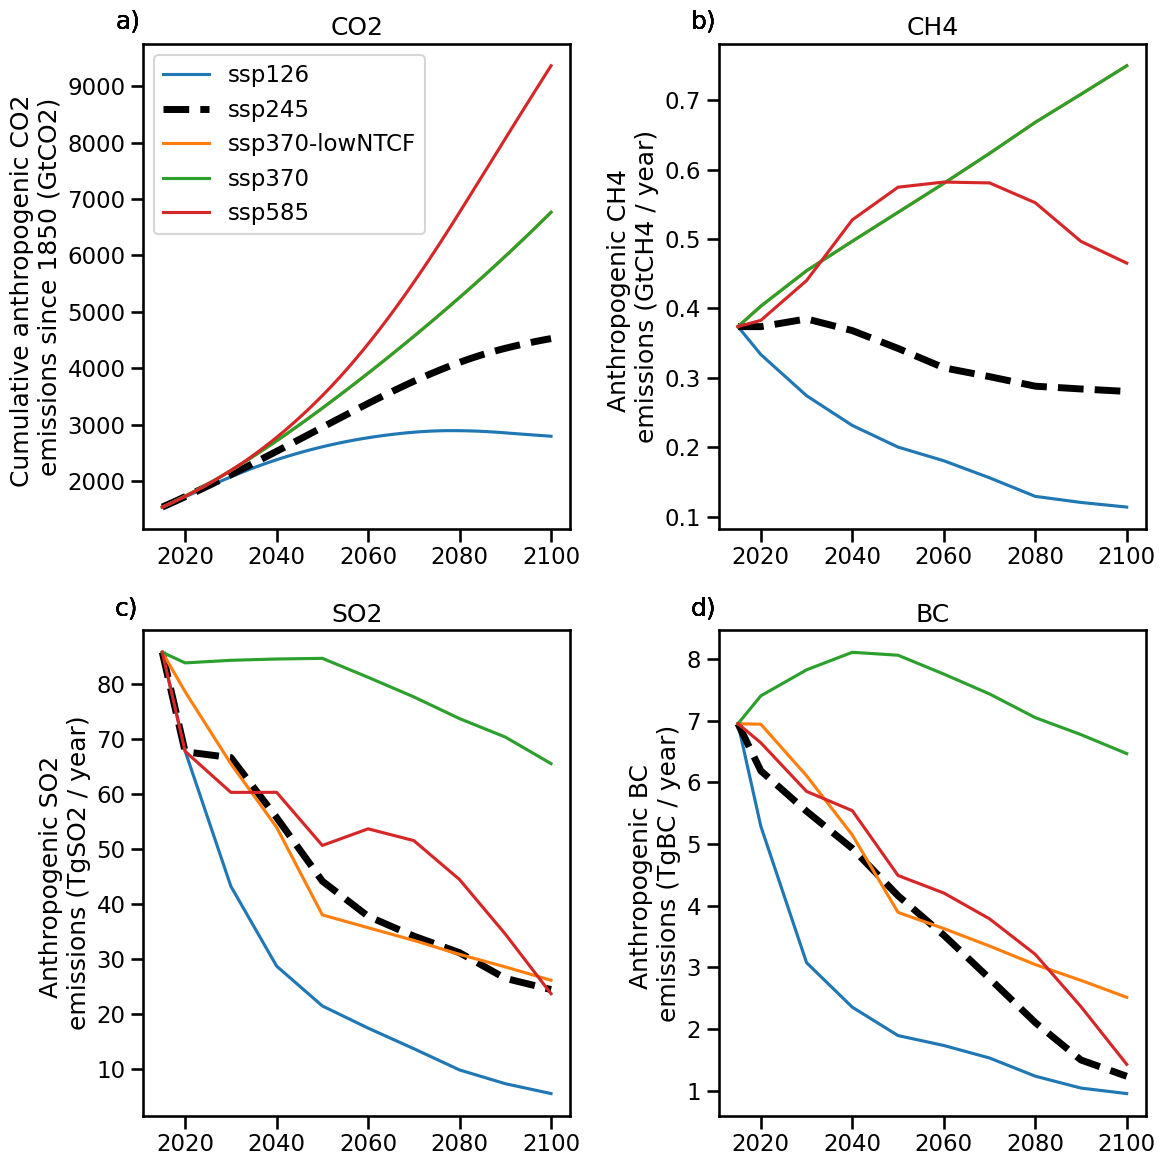
\includegraphics[width=5cm]{figure/input.png} }}%
     \qquad
     {{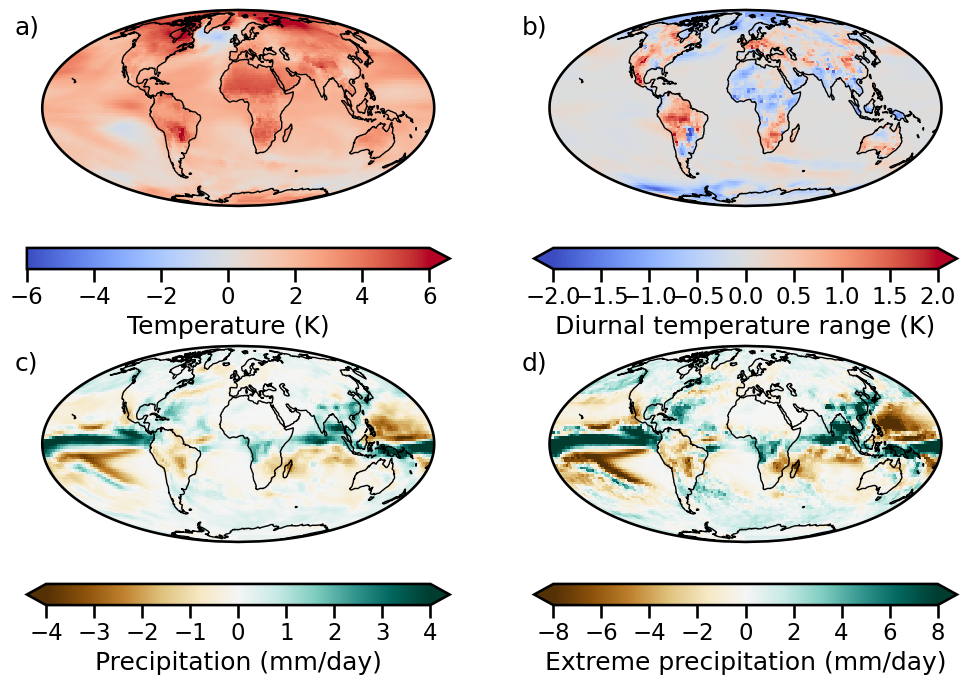
\includegraphics[width=6cm]{figure/output.png} }}%
     \caption{(a) Line Graphs of Input Variables from Multiple SSP (b) Map of Output Variables from SSP245}%
     \label{fig:example}%
\end{figure}


\section{Data}
Following the work of \cite{watson2022climatebench}, this paper will use the same training data from the Norwegian Earth System Model (NorESM2) which is generated data from simulations performed by the NorESM2 model. This was done as part of the sixth coupled model intercomparison project(CMIP6 ; Eyring et al.,2016 ). The data is used by the policymakers when deciding climate policies so that the emissions data that come from the NorESM2 and CMIP allow the improved ClimateBench Plus models to predict outcomes of different possible scenarios that align with the policymakers' want to reduce climate change. The data that is extracted from NorESM2 and CMIP are netcdfs which are multi-dimensional containing data on every latitude and longitude for the emissions and aerosols that we are looking at i.e Carbon Dioxide, Methane, Sulfur Dioxide, and Black Carbon and span from the 1850s to the end of 2100. 

The input variables include emission data of \textbf{CO$_{2}$}, \textbf{SO$_{2}$}, \textbf{CH$_{4}$}, and \textbf{Black Carbon} by different emission scenarios data and historical data. We took the global average of input variables CO$_{2}$ and CH$_{4}$ by year. We convert the units of SO$_{2}$ and Black Carbon into Tera gram and take the global sum. Through this process, we acquire the patterns of four different input variables from 2020 to 2100. The output variables are temperature (TAS), Precipitation (PR), 90th percentile precipitation (PR90), and daily diurnal temperature range (DTR). 

\subsection*{Data Preprocessing}
\label{sec:data_preprocessing}
For the base Neural Process we used a Sparse Representation of the data in order to reduce the data into 1 dimension. Where the context points are a mask of 10\% to 30\% of the training data from the geographical grid cells. The target points are the rest of the data. The data is then normalized to have a mean of 0 and a standard deviation of 1.

\begin{equation*}
    x \rightarrow (\text{lat}, \text{lon}, \text{time}, \text{aerosols input}) \quad y \rightarrow (\text{temperature}, \text{precipitation}, \text{DTR}, \text{PR90})
\end{equation*}

For the CNP models we use a multidimensional representation similar to the one in the Covolutional Neural Network baseline model in \cite{watson2022climatebench}. Where the dimensions are:

\begin{equation*}
    x \rightarrow (\text{time}, \text{aerosols input}, \text{lat}, \text{lon}) \quad y \rightarrow (\text{temperature}, \text{precipitation}, \text{DTR}, \text{PR90})
\end{equation*}

\section*{Neural Processes}
A Neural Process is a class of neural latent variable models which combines the best of both a Gaussian Process (GP) \cite*{rasmussen2006gaussian} and a Neural Network. The Neural Process (NP) \cite{garnelo2018neural} define a distribution over functions like GPs and are capable of rapid adaptation to new observations, and can also estimate the uncertainties. While at the same time are computationally efficient like Neural Networks and are able to adapt their their priors to the data, while as the same time also having the flexibility to model complex functions. 

A Neural Process is made up of two components, the encoder and the decoder. The encoder takes in the context points and encodes them into a latent representation. The decoder then takes the latent representation and the target points and decodes them into a distribution over the target points.

\begin{figure}[h!]
    \centering
    \includegraphics*[width=0.8\textwidth]{figure/np-model.png}
    \caption{Neural Process Model taken from \cite{garnelo2018neural}}
    \label{fig:np-model}
\end{figure}

With the flexibility of the Neural Process this allowed the construction of another variant of the Neural Process called the Convolutional Neural Process (CNP) \cite{gordon2020convolutional}. The CNP is a variant of the NP that uses a Convolutional Neural Network (CNN) to encode the context points. This allows the model to learn the spatial dependencies of the data. The CNP is able to learn the spatial dependencies of the data and is able to predict the target points based on the context points.

\section{Methods}
In this paper we used three different variations of the Neural Process Model to predict the global mean temperature, diurnal temperature range, and precipitation. The models are as follows:

\subsection*{Base Neural Process}
For a baseline model, we used a Neural Process model which takes in a sparse representation of the data, which reduces the higher dimensional spatial temporal data into a 1 dimensional representation. This simplifies the task removing the spatial dependencies and temporal dependencies of the data and making them independent of each other. This model is used to see how well the model can predict the data without the spatial and temporal dependencies.

The model takes in a sparse representation of the data \ref{sec:data_preprocessing} is passed through a linear Neural Network to encode the data into a latent representation with the context points. The latent representation is then passed through another linear Neural Network to decode the data into a distribution over the target points.

The architecture of the model is as follows:
% Add diagram of the model

\subsection*{Convolutional Neural Process}
The Convolutional Neural Process is a variant of the Neural Process that uses a Convolutional Neural Network to encode the context points. This allows the model to learn the spatial dependencies of the data. The model is able to learn the spatial dependencies of the data and is able to predict the target points based on the context points.

The model takes in a multidimensional representation of the data \ref{sec:data_preprocessing} is passed through a Convolutional Neural Network to encode the data into a latent representation with the context points. The latent representation is then passed through another Convolutional Neural Network to decode the data into a distribution over the target points.

The architecture of the model is as follows:

% Add diagram of the model

Details on the Neural Network layers can be found here 

\subsection*{Spherical Convolutional Neural Process}
Finally, we introduce the Spherical Convolutional Neural Process which is a variant of the Convolutional Neural Process that uses a Spherical Convolutional Neural Network to encode the context points. With the hopes to improve upon the Convolutional Neural Process by taking into account the spherical nature of the Earth when learning the spatial dependencies.

The model takes the same data as the Convolutional Neural Process and the architecture of the model is as follows:

% Add diagram of the model



\section{Evaluation against Benchmark Models}
\label{sec:evaluation_metric}
Following \cite{watson2022climatebench} we will also be using the $NRMSE_t$ from the paper which is defined as follows,
\begin{equation}
    NRMSE_s = \sqrt{\langle(|x_{i, j, t}|_t - |y_{i, j, t, n}|_{n, t})^2\rangle}/|\langle y_{i, j}\rangle|_{t, n}
\end{equation}
\begin{equation}
    NRMSE_g = \sqrt{|(\langle x_{i, j, t}\rangle - \langle|y_{i, j, t, n}|_n\rangle)^2|_t} / |\langle y_{i, j} \rangle|_{t, n}
\end{equation}
\begin{equation}
    NRMSE_t = NRMSE_s + \alpha \times NRMSE_g
\end{equation}

Where $NRMSE_s$ is the global mean root-mean squared error, and $NRMSE_g$ is $NRMSE$ in the global mean. The equation also includes a weighing function to take the decreasing grid-cell area towards the north and south poles which is defined as follows,
\begin{equation}
    \langle x_{i, j} \rangle = \frac{1}{N_{lat}N_{lon}}\sum_i^{N_{lat}}\sum_i^{N_{lon}} \cos(lat(i))x_{i, j}
\end{equation}
and the co-efficient $\alpha$ is chosen to be 5 from the ClimateBench paper, in order to provide equal weightage between the measures.

The reason, we are using this evaluation metric is to be able to compare directly the performances of our models against the models from the paper. And using the same evaluation metric will give us the most 1-1 comparison.

\section{Results}
Using the evaluation metric from \ref{sec:evaluation_metric} we are able to compare the performance of the models against the benchmark models from the ClimateBench paper. The results are as follows:

\begin{table}[t]
    \label{results-table}
    \begin{center}
        \begin{tabular}{lllll}
        \multicolumn{1}{c}{\bf Model}  &\multicolumn{1}{c}{\bf Temperature} & \multicolumn{1}{c}{\bf Precipitation} & \multicolumn{1}{c}{\bf DTR} & \multicolumn{1}{c}{\bf PR90}
        \\ \hline \\
        Base NP         & x \\
        CNP            & x \\
        Spherical CNP  & x \\
        GP             & x \\
        CNN             & x \\
        \end{tabular}
    \end{center}
    \caption{Comparison of the Neural Process Models against the Benchmark Models}
\end{table}

\section{Discussion}
neural processes benefit are does not require a lot of data, can be used for small datasets, can be used for high dimensional data, can be used for sequential data. Also good for few shot learning, works due to the context points.


\section{Conclusion}

\bibliography{iclr2024_conference}
\bibliographystyle{iclr2024_conference}

\appendix
\section{Model Architectures}

\subsection{Convolutional Neural Process}


\begin{table}[t]
    \caption{Sample table title}
    \label{sample-table}
    \begin{center}
        \begin{tabular}{ll}
        \multicolumn{1}{c}{\bf PART}  &\multicolumn{1}{c}{\bf DESCRIPTION}
        \\ \hline \\
        Dendrite         &Input terminal \\
        Axon             &Output terminal \\
        Soma             &Cell body (contains cell nucleus) \\
        \end{tabular}
    \end{center}
\end{table}


\subsection{Spherical Convolutional Neural Process}

\end{document}
